% Artigo adaptado ao modelo oficial da RITA (Revista de Inform\'atica Te\'orica e Aplicada).
% Para compilar: crie um projeto no Overleaf a partir do template "Revista de Inform\'atica
% Te\'orica e Aplicada - RITA" (https://www.overleaf.com/latex/templates/revista-de-informatica-teorica-e-aplicada-rita/fhxyfwnmhxzj),
% substitua RITAexemplo.tex por este arquivo e mantenha RITA.cls, artigo_bib.bib e figuras/.
\documentclass{RITA}
\usepackage[T1]{fontenc}
\usepackage{url}
\usepackage[brazilian,english]{babel}
\usepackage[utf8]{inputenc}
\usepackage{verbatim}
\usepackage{graphicx}
\usepackage[num]{abntex2cite}
\usepackage[a4paper]{geometry}

\title{An\'alise da rela\c{c}\~ao entre clima e desempenho agr\'icola em Varginha/MG: um estudo com pandas e dados p\'ublicos (2015--2025)}
\englishtitle{Climate and agricultural performance in Varginha/MG: a study with pandas and open data (2015--2025)}
\author{
  Luigi Miranda Penachio
    \footnote{Discente do curso de Computa\c{c}\~ao, Universidade Federal de Ci\^encia e Inova\c{c}\~ao de Minas Gerais (UFCIMG), Campus Varginha, Varginha/MG, Brasil. \texttt{luigimiranda2003@gmail.com, rafaelperim6@gmail.com}}
  \and
  Rafael de Paiva Perim
    \footnotemark[1]
  \and
  Eduardo Gomes Carvalho
    \footnote{Professor da UFCIMG, Campus Varginha, Varginha/MG, Brasil. \texttt{eduardogomes@cefetmg.br, marcelo.mussel@gmail.com}}
  \and
  Marcelo Mussel
    \footnotemark[2]
}
\RITAvolume{xx}
\RITAnumber{xx}
\RITAyear{2027}
\RITApagerange{xx-xx}

\begin{document}


\maketitle

\selectlanguage{brazilian}

\begin{abstract}
Este trabalho integra dados do INMET e do IBGE para avaliar se anomalias clim\'aticas explicam o desempenho da cafeicultura em Varginha/MG entre 2015 e 2025. Um pipeline em Python e Pandas agrega medi\c{c}\~oes da esta\c{c}\~ao A515 em indicadores anuais e janelas fenol\'ogicas e as junta aos rendimentos da PAM e ao rebanho da PPM, usando o ano como chave. Sequ\^encias longas de precipita\c{c}\~ao zero, identificadas como falha de sensor, foram imputadas pela mediana mensal. Correla\c{c}\~ao de Spearman, regress\~ao OLS, teste de Mann--Whitney e an\'alise de sensibilidade foram aplicados. A chuva anual apresentou $\rho=0,273$ ($p=0,416$) com o rendimento do caf\'e; a temperatura na flora\c{c}\~ao, $\rho=-0,418$ ($p=0,229$). Nenhuma rela\c{c}\~ao foi significativa a 5\%. Com onze anos de dados, n\~ao h\'a evid\^encia de efeito clim\'atico detect\'avel, o que refor\c{c}a a import\^ancia do controle de qualidade de sensores.
\end{abstract}

\begin{abstractinenglish}
\emph{This paper integrates meteorological data from the Brazilian National Institute of Meteorology (INMET) and municipal agricultural statistics from the Brazilian Institute of Geography and Statistics (IBGE) to assess whether climate anomalies explain coffee performance in Varginha, southern Minas Gerais, from 2015 to 2025. A reproducible Python/Pandas pipeline aggregates hourly records from station A515 into annual indicators and coffee phenological windows, and joins them to crop yields and cattle herd data using the year as key. Long zero-precipitation sequences, identified as sensor failure, were imputed with monthly medians. Spearman correlation, multiple linear regression, the Mann--Whitney test and a sensitivity analysis were applied. Annual rainfall showed $\rho=0.273$ ($p=0.416$) with coffee yield; temperature during flowering showed $\rho=-0.418$ ($p=0.229$). No relationship was significant at the 5\% level. With eleven annual observations, no detectable climatic effect was found, highlighting the importance of sensor quality control in public datasets.}
\end{abstractinenglish}

\begin{keywords}
An\'alise de dados. Cafeicultura. Dados abertos.
\end{keywords}

\begin{keywordsenglish}
\emph{Coffee. Data analysis. Open data.}
\end{keywordsenglish}

\section{Introdu\c{c}\~ao}

A cafeicultura brasileira tem papel central na economia rural e \'e sens\'ivel \`a distribui\c{c}\~ao de chuva e \`as oscila\c{c}\~oes t\'ermicas, especialmente nos est\'adios de flora\c{c}\~ao e forma\c{c}\~ao de frutos \cite{ipcc2021,aparecido2016}. No Sul de Minas Gerais, a colheita do caf\'e ar\'abica ocorre principalmente entre abril e agosto, enquanto a flora\c{c}\~ao acontece na primavera do ano anterior. Essa defasagem exige que o analista escolha janelas temporais alinhadas ao ciclo da cultura, e n\~ao apenas indicadores anuais de precipita\c{c}\~ao e temperatura \cite{meireles2009}.

Varginha/MG \'e um dos principais polos cafeeiros do Sul de Minas e conta com uma esta\c{c}\~ao autom\'atica do INMET (c\'odigo A515) com s\'erie cont\'inua no per\'iodo analisado. Ao mesmo tempo, o IBGE divulga anualmente o rendimento municipal da lavoura por meio da Pesquisa Agr\'icola Municipal (PAM) e o efetivo de rebanhos pela Pesquisa da Pecu\'aria Municipal (PPM). A combina\c{c}\~ao dessas fontes permite construir um painel municipal anual com informa\c{c}\~ao clim\'atica e agron\^omica \cite{inmet2026,ibgePAM2025,ibgePPM2025}.

Apesar da disponibilidade dos dados, ainda s\~ao raros os estudos reproduz\'iveis que documentem, em c\'odigo aberto, a limpeza das s\'eries meteorol\'ogicas, o tratamento de falhas de sensores e a jun\c{c}\~ao com estat\'isticas agropecu\'arias. Este artigo preenche essa lacuna e responde a tr\^es perguntas: (i) anomalias de precipita\c{c}\~ao e temperatura explicam varia\c{c}\~oes anuais do rendimento do caf\'e em Varginha? (ii) janelas fenol\'ogicas apresentam associa\c{c}\~ao mais forte do que a m\'edia anual? (iii) o rebanho bovino responde \`a precipita\c{c}\~ao com defasagem de um ano?

As hip\'oteses iniciais eram de associa\c{c}\~ao positiva entre chuva e rendimento, negativa entre calor na flora\c{c}\~ao e rendimento, e positiva entre chuva defasada e rebanho. Os resultados, como se ver\'a, n\~ao confirmam nenhuma delas de forma significativa.

\section{Trabalhos relacionados}

Victorino \cite{victorino2015} adaptou um modelo agrometeorol\'ogico de previs\~ao de produtividade para Lavras e Varginha. Os modelos foram sens\'iveis ao d\'eficit h\'idrico entre novembro e abril, e as vari\'aveis associadas \`a flora\c{c}\~ao n\~ao foram significativas. Aparecido et al.\ \cite{aparecido2016} calibraram modelos de regress\~ao m\'ultipla para seis regi\~oes produtoras de Minas Gerais, com anteced\^encia de at\'e seis meses, e conclu\'iram que no Sul de Minas a produtividade \'e controlada por m\'ultiplos elementos meteorol\'ogicos, enquanto no Cerrado Mineiro o regime h\'idrico domina.

Meireles e Japiass\'u \cite{meireles2009} descreveram a fenologia do cafeeiro em Varginha e mostraram que a aus\^encia de chuvas entre setembro e outubro reduziu a dorm\^encia e o crescimento dos ramos, prejudicando a flora\c{c}\~ao. Gomes et al.\ \cite{gomes2026} analisaram tend\^encias de temperatura e precipita\c{c}\~ao entre 1984 e 2023 em duas unidades produtivas do Sul de Minas e encontraram correla\c{c}\~oes de sinais opostos entre elas, atribu\'idas a microclima, uso e cobertura do solo.

Tais trabalhos empregam s\'eries de esta\c{c}\~oes especializadas, dados de cooperativas ou unidades produtivas espec\'ificas. Este artigo difere ao usar somente bases p\'ublicas e um pipeline de c\'odigo aberto, explicitando o controle de qualidade e a incerteza associada a uma amostra de apenas onze anos.

\section{Materiais e m\'etodos}

\subsection{Local de estudo e bases de dados}

O recorte espacial \'e o munic\'ipio de Varginha, c\'odigo IBGE 3170701, localizado no Sul de Minas Gerais. A esta\c{c}\~ao autom\'atica A515, operada pelo INMET, est\'a dentro do munic\'ipio, nas coordenadas $-21{,}5664^\circ$ de latitude e $-45{,}4042^\circ$ de longitude, com altitude de aproximadamente 950 m. O per\'iodo analisado vai de 2015 a 2025.

Foram usadas tr\^es bases p\'ublicas, resumidas na Tabela~\ref{tab:bases}. Os arquivos anuais do INMET s\~ao ZIPs com um CSV hor\'ario por esta\c{c}\~ao; as s\'eries do IBGE foram obtidas pela API SIDRA. A PAM fornece o rendimento m\'edio em kg/ha para o caf\'e em gr\~ao (c\'odigo 40139), milho (40122) e soja (40124). A PPM fornece o efetivo de bovinos em 31 de dezembro (c\'odigo 2670).

\begin{table}[ht]
\begin{center}
\caption{Bases de dados, unidades observadas e vari\'aveis utilizadas.}
\label{tab:bases}
\begin{tabular}{llll}
\hline
Base & Fonte & Unidade & Vari\'aveis \\
\hline
INMET BDMEP & ZIP anual A515 & hora/dia/m\^es/ano & precipita\c{c}\~ao, temperatura, dias com $T_{\max}>35\,^\circ$C \\
IBGE PAM & SIDRA 5457 & munic\'ipio/ano & rendimento de caf\'e, milho e soja (kg/ha) \\
IBGE PPM & SIDRA 3939 & munic\'ipio/ano & efetivo de bovinos (cabe\c{c}as) \\
\hline
\end{tabular}
\end{center}
\end{table}

\subsection{Chave de jun\c{c}\~ao}

A chave adotada foi o \textbf{ano}, com esta\c{c}\~ao e munic\'ipio como atributos fixos. A justificativa \'e direta: a esta\c{c}\~ao A515 pertence ao pr\'oprio munic\'ipio de Varginha, e PAM e PPM tamb\'em t\^em unidade municipal. N\~ao h\'a, portanto, necessidade de jun\c{c}\~ao espacial entre bases distintas. O uso do ano garante que a safra de refer\^encia do IBGE seja pareada com um ano meteorol\'ogico completo. Para as janelas que envolvem a flora\c{c}\~ao, foi usado o ano anterior ao da colheita, conforme o ciclo descrito por Meireles e Japiass\'u \cite{meireles2009}.

\subsection{Pr\'e-processamento meteorol\'ogico}

Os CSVs do INMET apresentam dois layouts. At\'e 2018, as datas usam o formato \texttt{AAAA-MM-DD}, as horas \texttt{HH:MM} e o valor ausente \'e codificado como $-9999$. A partir de 2019, as datas usam \texttt{AAAA/MM/DD}, as horas \texttt{HHMM UTC} e as c{\'e}lulas vazias indicam aus\^encia. Ambos foram normalizados no pipeline. Foram descartados dias com menos de seis horas v\'alidas e meses com menos de quinze dias v\'alidos.

A an\'alise de qualidade revelou um problema cr\'itico: a esta\c{c}\~ao registrou $0$ mm de precipita\c{c}\~ao em sequ\^encias de tr\^es a oito meses (mai--jul/2019, mai--jul/2022, mai--dez/2023 e jan--mar/2024), incompat\'iveis com a climatologia local: em maio e junho as medianas s\~ao de 24,6 e 27,1 mm, e em dezembro, de 219,2 mm. Tamb\'em havia meses ausentes (ago/2016 e dez/2025). Como n\~ao consultamos a documenta\c{c}\~ao do INMET sobre esses eventos, tratamos esses registros como suspeitos: sequ\^encias de pelo menos tr\^es meses com precipita\c{c}\~ao inferior a 1 mm foram marcadas como falha de sensor e, junto com os meses ausentes, imputadas pela mediana mensal calculada sobre os demais anos. Foram 19 meses imputados, oito deles apenas em 2023. Cada m\^es imputado foi sinalizado em uma coluna bin\'aria do painel.

\subsection{Indicadores clim\'aticos e janelas fenol\'ogicas}

A agrega\c{c}\~ao foi feita de hora para dia, de dia para m\^es e de m\^es para ano. Os indicadores anuais s\~ao: precipita\c{c}\~ao acumulada, temperatura m\'edia, temperatura m\'axima m\'edia e n\'umero de dias com m\'axima acima de $35\,^\circ$C. As janelas fenol\'ogicas consideradas foram: flora\c{c}\~ao (setembro a novembro do ano anterior), frutifica\c{c}\~ao (dezembro do ano anterior a mar\c{c}o do ano da colheita), colheita (abril a agosto do ano da colheita) e janeiro do ano da colheita, esta \'ultima de forma explorat\'oria. Para cada vari\'avel, calculou-se a anomalia z em rela\c{c}\~ao \`a m\'edia e ao desvio-padr\~ao do per\'iodo 2015--2025.

\subsection{Dados agropecu\'arios e outliers}

Os rendimentos e o rebanho foram extra\'idos no n\'ivel municipal pela API SIDRA. O cabe\c{c}alho do JSON retornado alterna entre nomes leg\'iveis e c\'odigos como \texttt{D1N} e \texttt{D4N}; por isso o extrator normaliza as colunas por posi\c{c}\~ao. Valores \texttt{-} ou \texttt{...} foram convertidos em ausentes. Aos percentis 1\% e 99\% das vari\'aveis de produ\c{c}\~ao aplicou-se winsoriza\c{c}\~ao, depois do c\'alculo das anomalias, para evitar que observa\c{c}\~oes extremas distorcessem os coeficientes.

\subsection{T\'ecnicas estat\'isticas}

Foram aplicadas quatro t\'ecnicas: (1) correla\c{c}\~ao de Pearson e Spearman entre anomalias clim\'aticas e rendimentos, com p-valores; (2) regress\~ao linear OLS com modelos de uma ou duas vari\'aveis, incluindo um termo quadr\'atico da chuva anual; (3) teste n\~ao param\'etrico de Mann--Whitney comparando o rendimento em anos secos e chuvosos; e (4) regress\~ao do rebanho bovino contra a anomalia de chuva do ano anterior. Como an\'alise complementar, repetiram-se as correla\c{c}\~oes sem os anos com falhas longas de precipita\c{c}\~ao. As an\'alises usaram Pandas \cite{mckinney2010}, SciPy \cite{virtanen2020}, Statsmodels \cite{seabold2010}, Matplotlib e Seaborn \cite{waskom2021}. Todo o c\'odigo, os dados intermedi\'arios e as figuras est\~ao dispon\'iveis em reposit\'orio p\'ublico: \url{https://github.com/LuigiPenachio/clima-cafe-varginha-pandas}.

\section{Resultados}

\subsection{Climatologia e estat\'istica descritiva}

A Figura~\ref{fig:mapa} mostra a localiza\c{c}\~ao do munic\'ipio e da esta\c{c}\~ao. A Figura~\ref{fig:clima} apresenta a climatologia mensal: dezembro \'e o m\^es mais chuvoso, seguido de janeiro, e julho e agosto s\~ao os mais secos, padr\~ao compat\'ivel com o regime do Sul de Minas.

\begin{figure}[ht]
\begin{center}
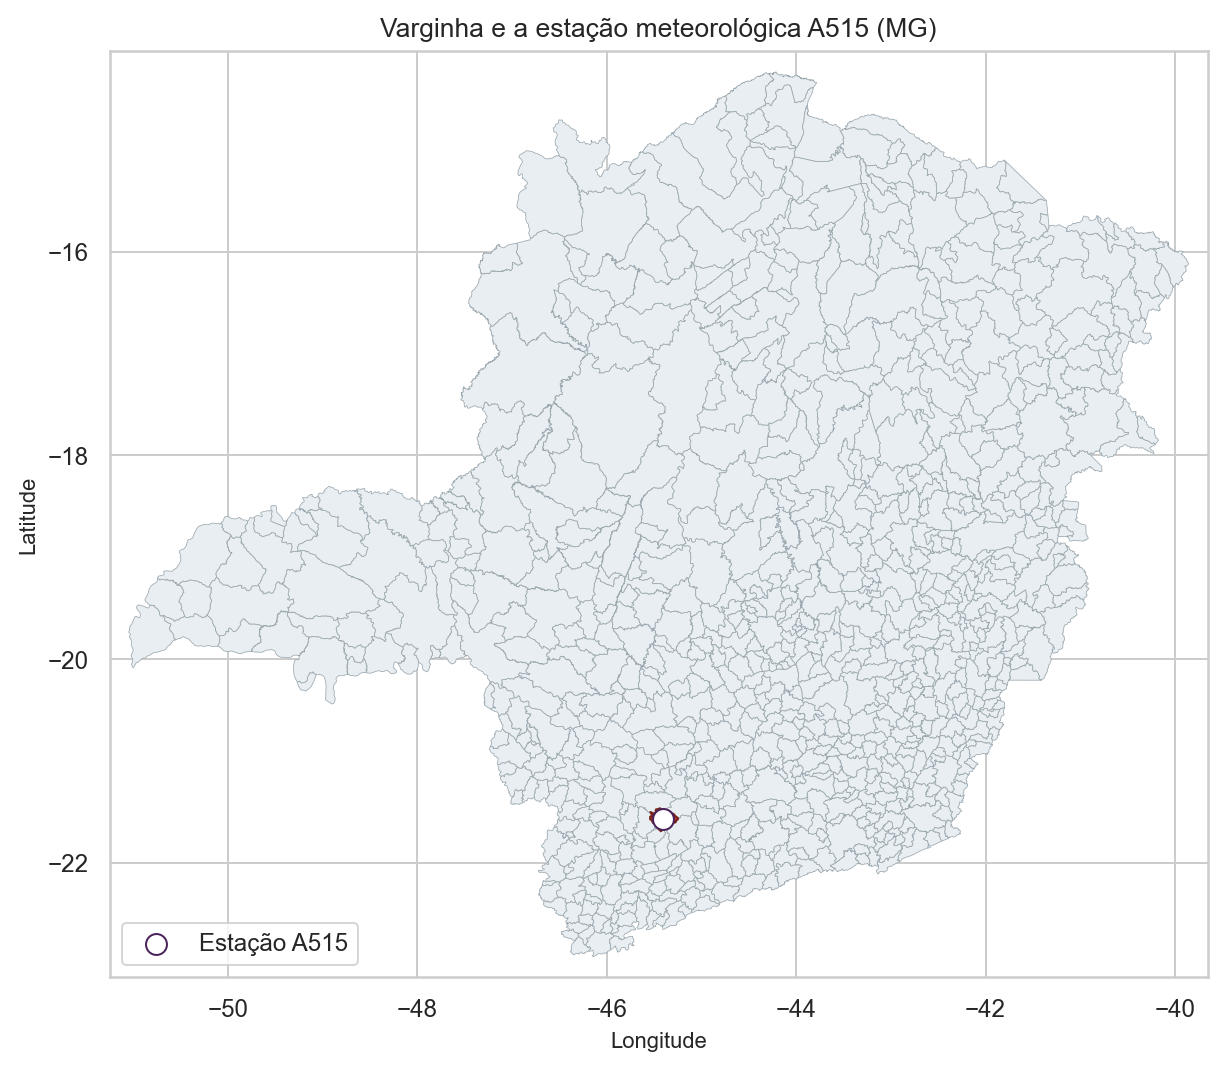
\includegraphics[width=.75\textwidth]{figuras/01_mapa_varginha.png}
\caption{Localiza\c{c}\~ao de Varginha em Minas Gerais e da esta\c{c}\~ao autom\'atica A515.}
\label{fig:mapa}
\end{center}
\end{figure}

\begin{figure}[ht]
\begin{center}
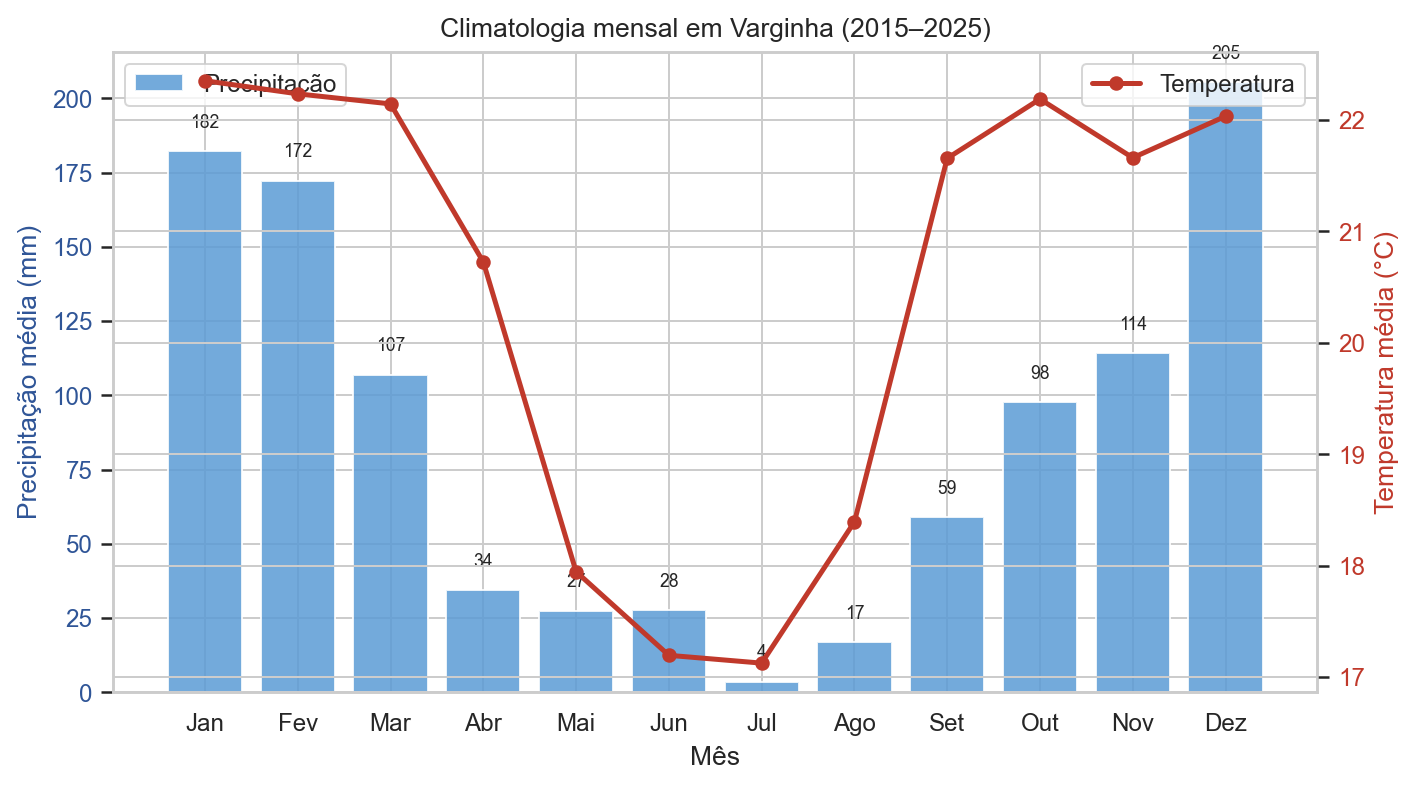
\includegraphics[width=.9\textwidth]{figuras/02_climograma.png}
\caption{Climatologia mensal de precipita\c{c}\~ao e temperatura em Varginha, m\'edia de 2015--2025, ap\'os imputa\c{c}\~ao.}
\label{fig:clima}
\end{center}
\end{figure}

A Tabela~\ref{tab:desc} resume as vari\'aveis. A precipita\c{c}\~ao anual m\'edia ap\'os imputa\c{c}\~ao foi de 1047,6 mm, com m\'inimo de 727,8 mm e m\'aximo de 1476,2 mm. A temperatura m\'edia foi de $20{,}47\,^\circ$C e o n\'umero m\'edio de dias com $T_{\max}>35\,^\circ$C foi 1,82. O rendimento m\'edio do caf\'e foi de 1567,24 kg/ha (1038 a 2121,6 kg/ha), do milho 7187 kg/ha e da soja 3844 kg/ha. O rebanho bovino m\'edio foi de 16\,481 cabe\c{c}as.

\begin{table}[ht]
\begin{center}
\caption{Estat\'istica descritiva do painel de Varginha (2015--2025), ap\'os winsoriza\c{c}\~ao.}
\label{tab:desc}
\begin{tabular}{lrrrr}
\hline
Vari\'avel & M\'edia & Desvio & M\'inimo & M\'aximo \\
\hline
Precipita\c{c}\~ao anual (mm) & 1047,6 & 245,4 & 727,8 & 1476,2 \\
Temperatura m\'edia ($^\circ$C) & 20,47 & 0,41 & 19,93 & 21,37 \\
Dias com $T_{\max}>35\,^\circ$C & 1,82 & 2,75 & 0 & 8 \\
Rendimento do caf\'e (kg/ha) & 1567,2 & 372,9 & 1038,0 & 2121,6 \\
Rendimento do milho (kg/ha) & 7187,0 & 981,5 & 6000,0 & 8690,0 \\
Rendimento da soja (kg/ha) & 3844,2 & 269,8 & 3600,0 & 4361,0 \\
Rebanho bovino (cabe\c{c}as) & 16\,481 & 975 & 14\,906 & 18\,177 \\
\hline
\end{tabular}
\end{center}
\end{table}

A Figura~\ref{fig:serie} mostra a evolu\c{c}\~ao do rendimento do caf\'e e da anomalia de chuva. Observa-se que os anos de maior rendimento n\~ao coincidem sistematicamente com os anos mais chuvosos: 2017 e 2018 tiveram rendimentos altos com anomalias de chuva pr\'oximas de zero, enquanto 2023 teve forte anomalia positiva e rendimento apenas moderado.

\begin{figure}[ht]
\begin{center}
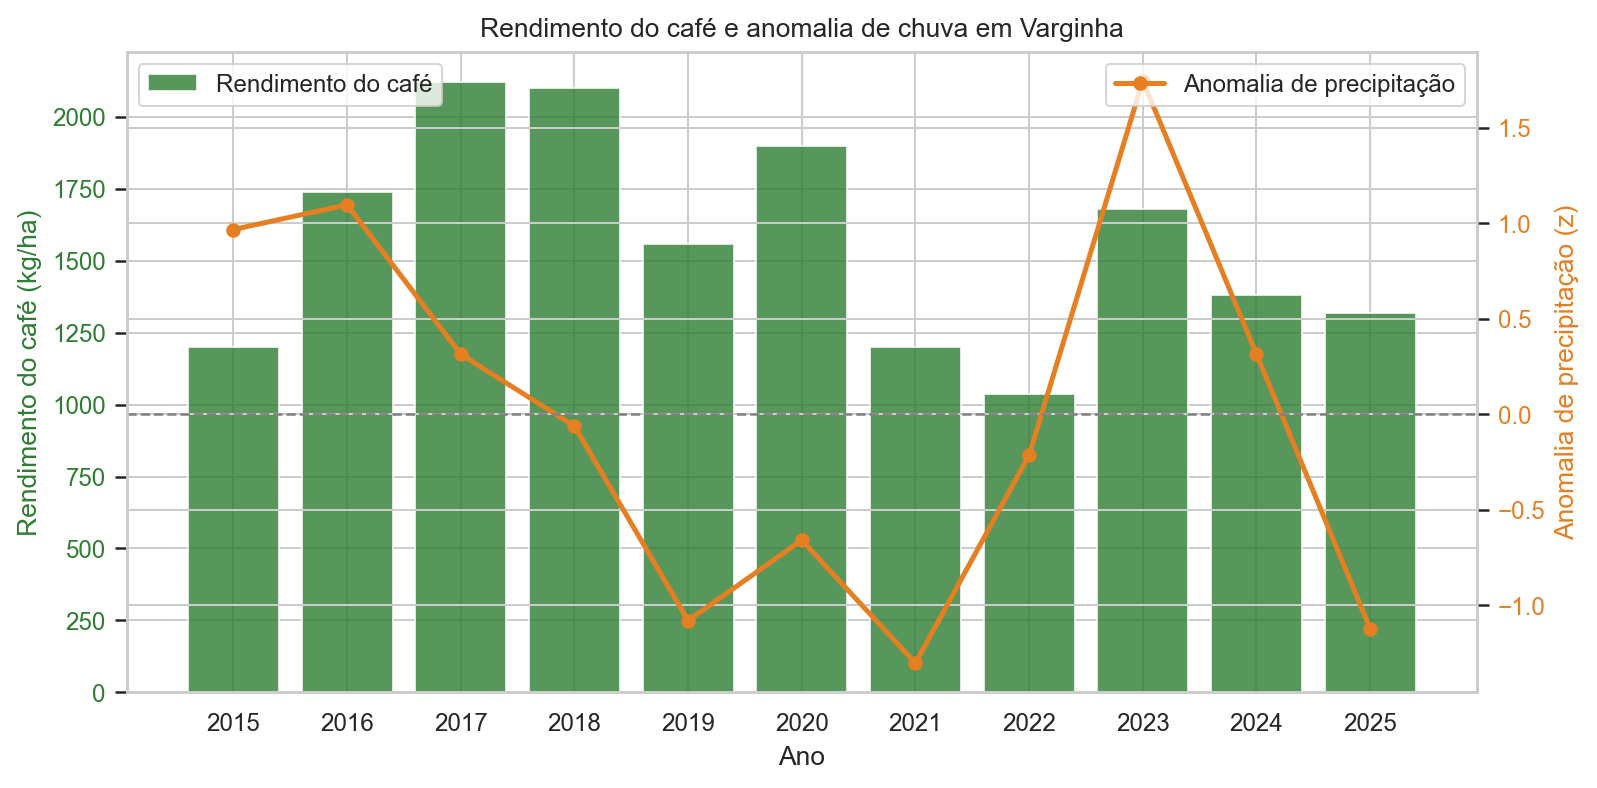
\includegraphics[width=.9\textwidth]{figuras/03_serie_rendimento_clima.png}
\caption{Rendimento do caf\'e (barras) e anomalia anual de precipita\c{c}\~ao (linha), 2015--2025.}
\label{fig:serie}
\end{center}
\end{figure}

\subsection{Correla\c{c}\~oes}

A Tabela~\ref{tab:corr} apresenta as correla\c{c}\~oes. A chuva anual correlacionou-se com o rendimento do caf\'e com $\rho=0{,}273$ ($p=0{,}4160$). A chuva na frutifica\c{c}\~ao teve $\rho=0{,}406$ ($p=0{,}2443$) e a chuva na flora\c{c}\~ao $\rho=0{,}224$ ($p=0{,}5334$). A temperatura na flora\c{c}\~ao apresentou $\rho=-0{,}418$ ($p=0{,}2291$), na dire\c{c}\~ao esperada, por\'em n\~ao significativa. A temperatura m\'edia anual e o n\'umero de dias quentes foram praticamente nulos.

\begin{table}[ht]
\begin{center}
\caption{Correla\c{c}\~oes de Spearman e Pearson entre indicadores clim\'aticos e anomalia do rendimento do caf\'e.}
\label{tab:corr}
\begin{tabular}{lcccc}
\hline
Vari\'avel & $n$ & $\rho$ de Spearman & $p$ & $r$ de Pearson \\
\hline
Chuva na frutifica\c{c}\~ao & 10 & 0,406 & 0,2443 & 0,359 \\
Chuva anual & 11 & 0,273 & 0,4160 & 0,206 \\
Chuva na colheita & 11 & 0,187 & 0,5824 & 0,206 \\
Chuva na flora\c{c}\~ao & 10 & 0,224 & 0,5334 & 0,327 \\
Temperatura m\'edia & 11 & $-0{,}005$ & 0,9894 & $-0{,}120$ \\
Dias quentes & 11 & $-0{,}048$ & 0,8879 & 0,157 \\
Temperatura na flora\c{c}\~ao & 10 & $-0{,}418$ & 0,2291 & $-0{,}360$ \\
\hline
\end{tabular}
\end{center}
\end{table}

O mapa de calor da Figura~\ref{fig:heat} confirma que nenhuma vari\'avel clim\'atica apresenta associa\c{c}\~ao forte com o rendimento do caf\'e. A correla\c{c}\~ao entre chuva na frutifica\c{c}\~ao e rendimento do milho foi de $r=0{,}57$, e a do rebanho com chuva defasada foi pr\'oxima de zero ($r=0{,}03$).

\begin{figure}[ht]
\begin{center}
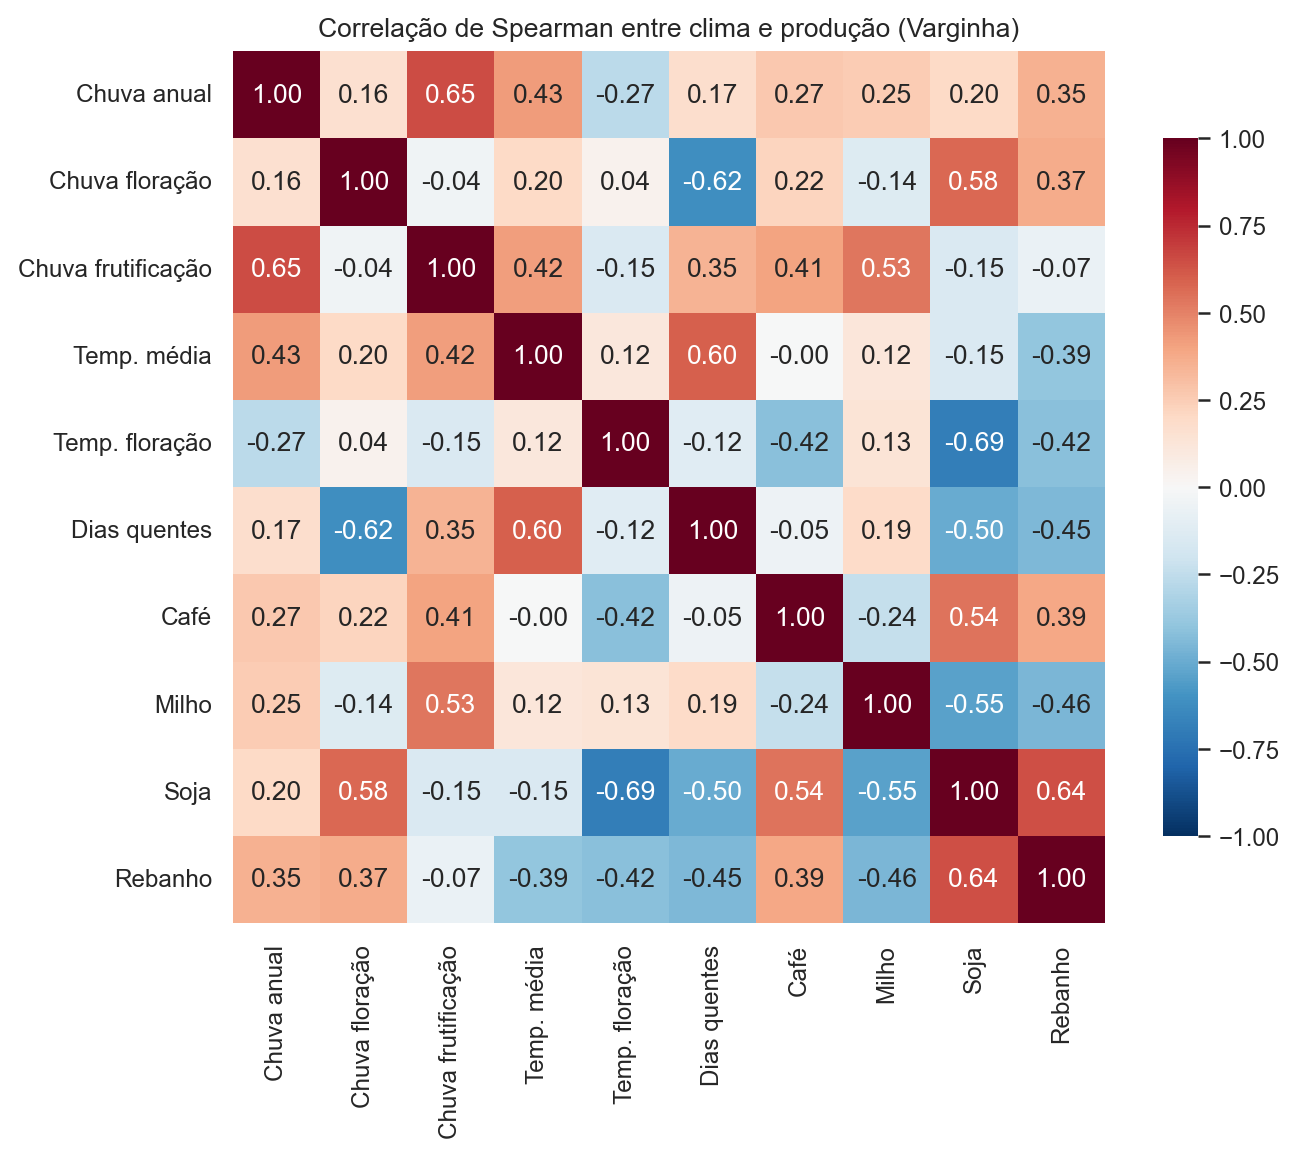
\includegraphics[width=.9\textwidth]{figuras/08_heatmap_correlacoes.png}
\caption{Matriz de correla\c{c}\~ao de Spearman entre clima e produ\c{c}\~ao agropecu\'aria.}
\label{fig:heat}
\end{center}
\end{figure}

A an\'alise mensal explorat\'oria da Figura~\ref{fig:mensais} indicou $\rho=0{,}446$ ($p=0{,}169$) para janeiro e $\rho=-0{,}405$ ($p=0{,}217$) para dezembro. Como doze coeficientes foram testados, esses valores n\~ao devem ser interpretados como descobertas, mas como hip\'oteses a serem avaliadas em s\'eries mais longas.

\begin{figure}[ht]
\begin{center}
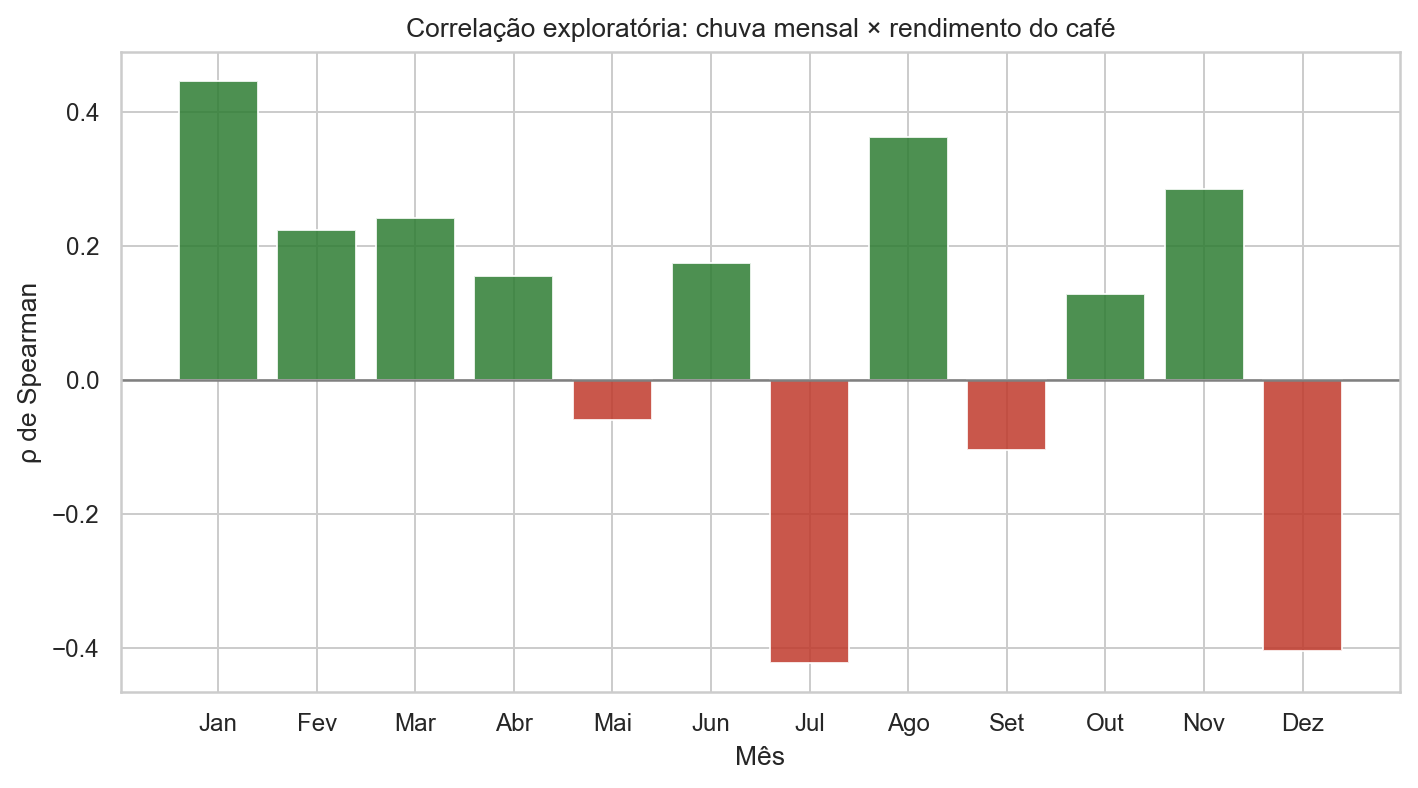
\includegraphics[width=.9\textwidth]{figuras/10_janelas_mensais.png}
\caption{Correla\c{c}\~ao de Spearman entre a anomalia de precipita\c{c}\~ao de cada m\^es e o rendimento do caf\'e (explorat\'orio).}
\label{fig:mensais}
\end{center}
\end{figure}

\subsection{Modelos de regress\~ao}

A Tabela~\ref{tab:ols} mostra os quatro modelos estimados. O modelo com apenas a anomalia de chuva anual explicou $4{,}3\%$ da varia\c{c}\~ao do rendimento ($p=0{,}5425$). A inclus\~ao da chuva na frutifica\c{c}\~ao e do calor na flora\c{c}\~ao elevou $R^2$ para $0{,}205$, mas o teste F global n\~ao foi significativo ($p=0{,}4472$). O modelo quadr\'atico tamb\'em n\~ao foi significativo ($p=0{,}6778$), assim como o modelo com a chuva de janeiro ($p=0{,}4050$).

\begin{table}[ht]
\begin{center}
\caption{Resultados dos modelos OLS para a anomalia do rendimento do caf\'e.}
\label{tab:ols}
\begin{tabular}{lrrr}
\hline
Modelo & $R^2$ & $R^2$ ajustado & $p$ do teste F \\
\hline
M1: chuva anual & 0,043 & $-0{,}064$ & 0,5425 \\
M2: chuva na frutifica\c{c}\~ao + calor na flora\c{c}\~ao & 0,205 & $-0{,}022$ & 0,4472 \\
M3: termo quadr\'atico da chuva anual & 0,093 & $-0{,}134$ & 0,6778 \\
M4: chuva de janeiro & 0,078 & $-0{,}024$ & 0,4050 \\
\hline
\end{tabular}
\end{center}
\end{table}

A Figura~\ref{fig:scatter} ilustra o modelo M1: a linha ajustada tem inclina\c{c}\~ao positiva, por\'em os pontos est\~ao dispersos e o intervalo de confian\c{c}a inclui a hip\'otese nula. A Figura~\ref{fig:calor} mostra a rela\c{c}\~ao negativa, tamb\'em n\~ao significativa, entre calor na flora\c{c}\~ao e rendimento.

\begin{figure}[ht]
\begin{center}
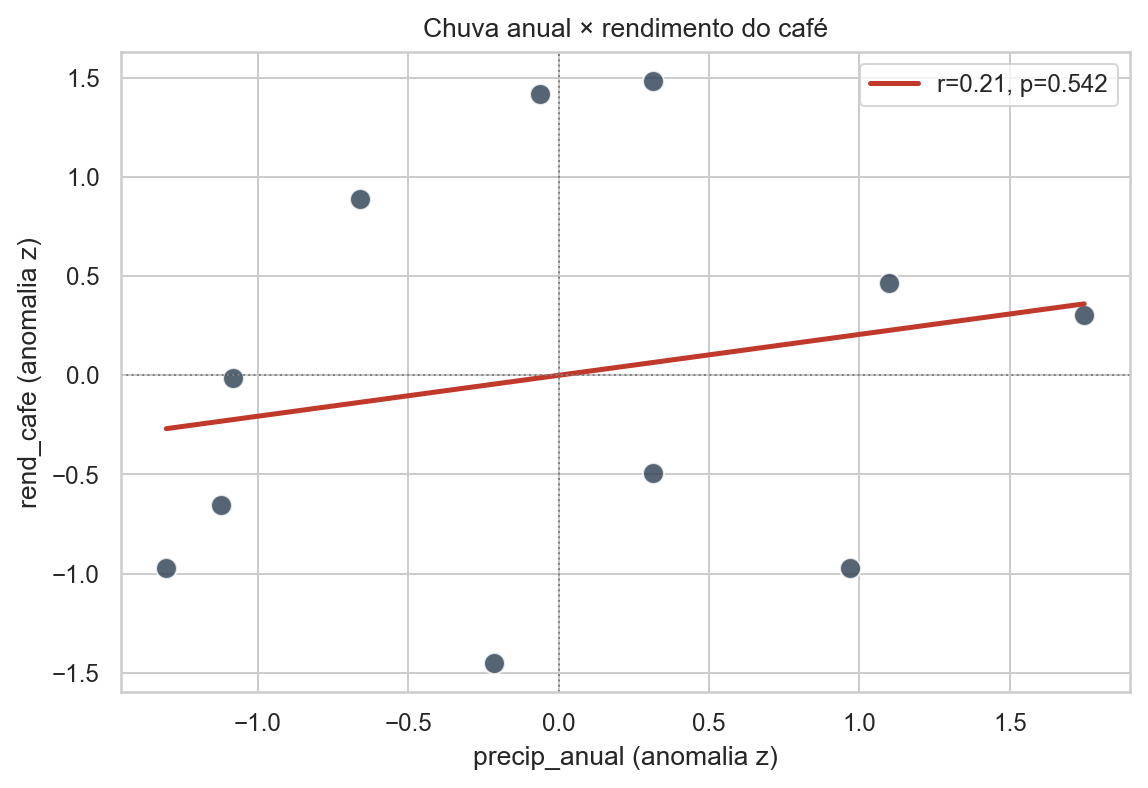
\includegraphics[width=.8\textwidth]{figuras/04_dispersao_chuva_cafe.png}
\caption{Anomalia de precipita\c{c}\~ao anual versus anomalia do rendimento do caf\'e, com linha ajustada.}
\label{fig:scatter}
\end{center}
\end{figure}

\begin{figure}[ht]
\begin{center}
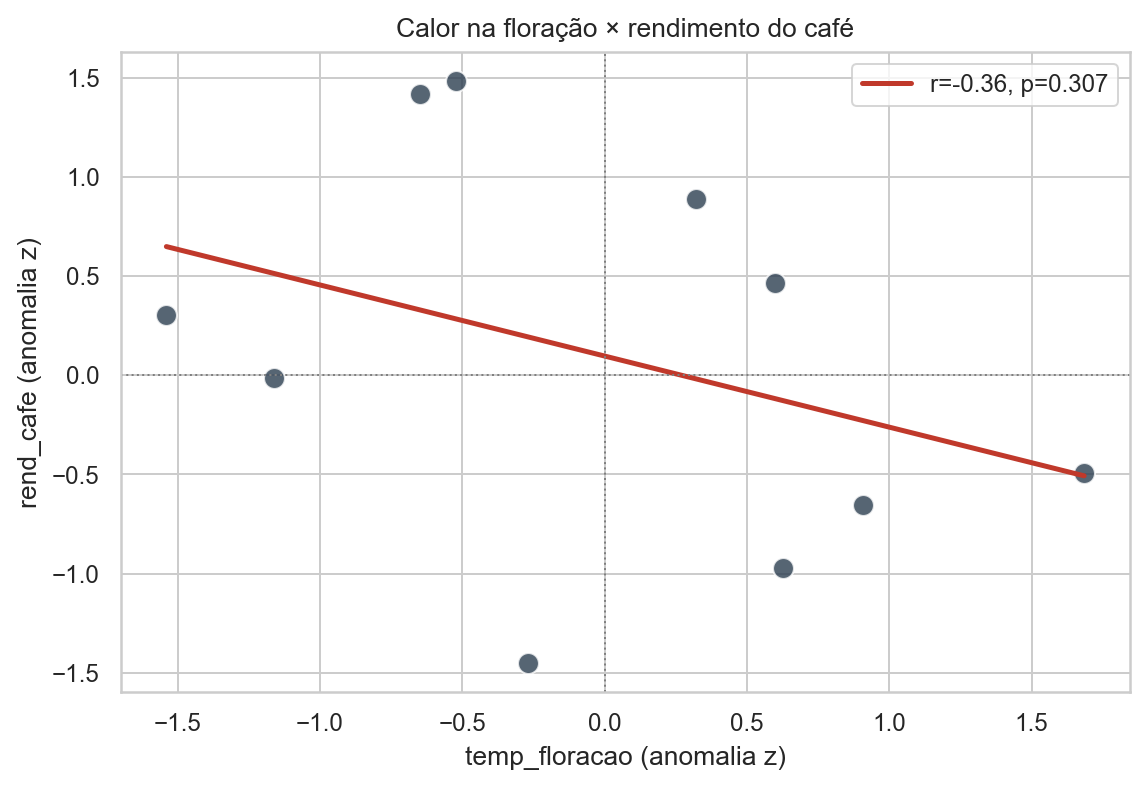
\includegraphics[width=.8\textwidth]{figuras/05_dispersao_calor_cafe.png}
\caption{Anomalia de temperatura na flora\c{c}\~ao versus anomalia do rendimento do caf\'e.}
\label{fig:calor}
\end{center}
\end{figure}

\subsection{Teste de hip\'oteses e sensibilidade}

O teste de Mann--Whitney comparou o rendimento de quatro anos secos, quatro normais e tr\^es chuvosos, definidos por limiares de $\pm 0{,}5$ na anomalia de precipita\c{c}\~ao. N\~ao houve diferen\c{c}a ($U=5{,}5$; $p=1{,}0000$), como mostra a Figura~\ref{fig:box}.

\begin{figure}[ht]
\begin{center}
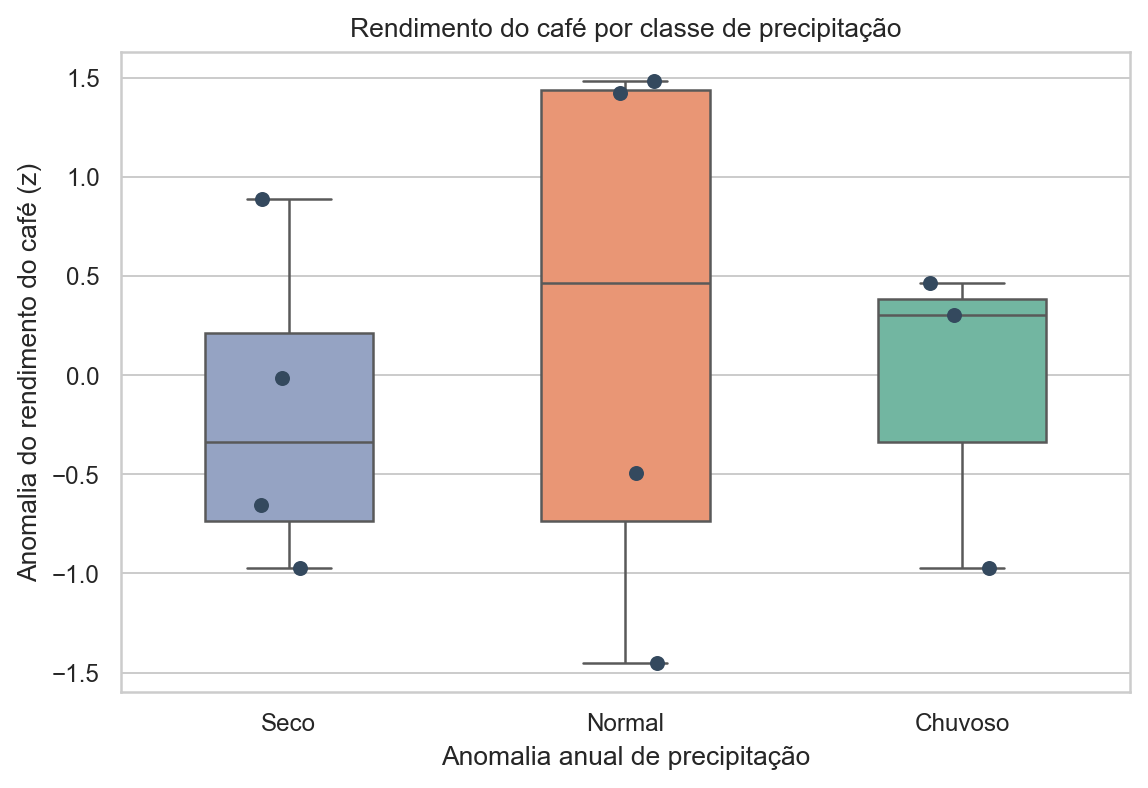
\includegraphics[width=.8\textwidth]{figuras/06_boxplot_anos_secos.png}
\caption{Distribui\c{c}\~ao da anomalia do rendimento do caf\'e por classe de precipita\c{c}\~ao anual.}
\label{fig:box}
\end{center}
\end{figure}

A regress\~ao do rebanho bovino contra a chuva do ano anterior resultou em $\beta=0{,}029$, $R^2=0{,}001$ e $p=0{,}9395$, sem evid\^encia de associa\c{c}\~ao (Figura~\ref{fig:rebanho}). Vale registrar que, antes da corre\c{c}\~ao dos meses com falha de sensor, essa mesma regress\~ao apontava $R^2=0{,}54$ e $p=0{,}015$. A mudan\c{c}a de conclus\~ao mostra como artefatos de sensor podem gerar resultados esp\'urios em s\'eries curtas.

\begin{figure}[ht]
\begin{center}
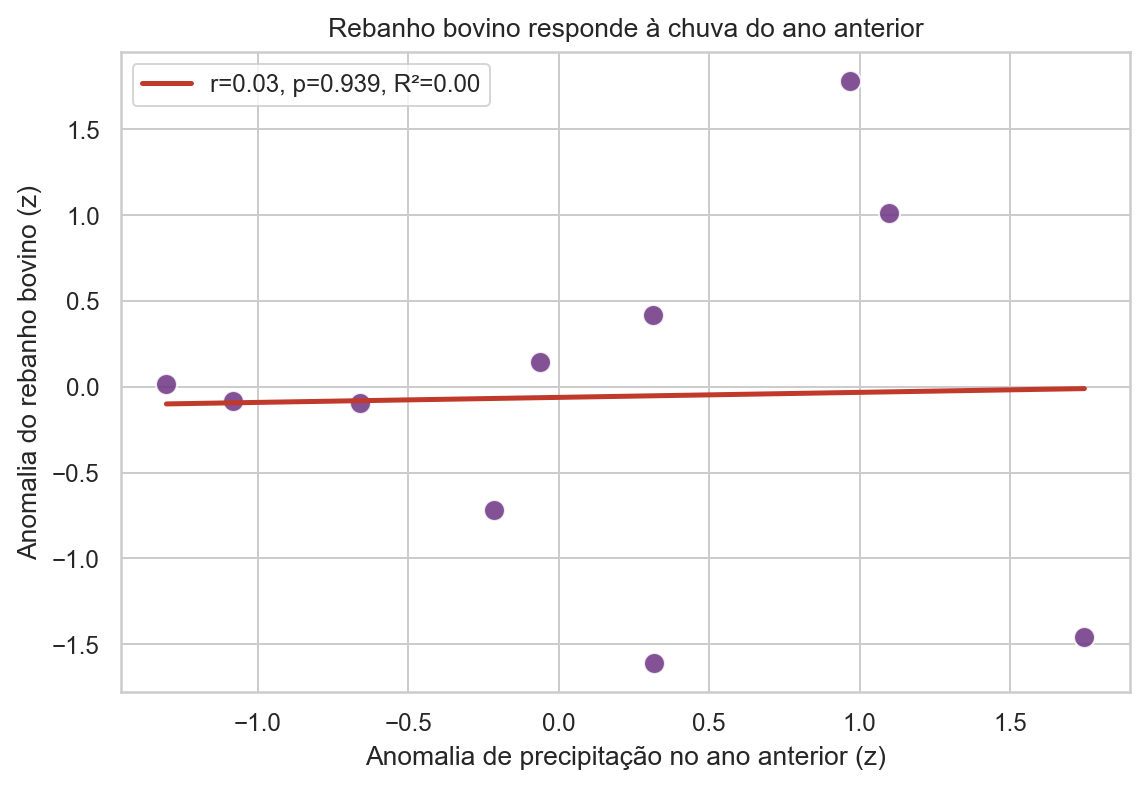
\includegraphics[width=.8\textwidth]{figuras/09_rebanho_chuva_atrasada.png}
\caption{Rebanho bovino versus anomalia de precipita\c{c}\~ao do ano anterior, ap\'os imputa\c{c}\~ao.}
\label{fig:rebanho}
\end{center}
\end{figure}

A an\'alise de sensibilidade excluiu os anos com sequ\^encias imputadas, restando 2015, 2016, 2017, 2018, 2020, 2021 e 2025. A correla\c{c}\~ao entre chuva anual e rendimento permaneceu nula ($\rho=0{,}234$; $p=0{,}6132$; $n=7$). A correla\c{c}\~ao entre temperatura na flora\c{c}\~ao e rendimento passou a ser forte e significativa ($\rho=-0{,}886$; $p=0{,}0188$), por\'em com apenas seis pares v\'alidos, por quest\~ao de defasagem da janela. Esse resultado \'e explorat\'orio e n\~ao deve ser tratado como confirma\c{c}\~ao da hip\'otese.

\subsection{S\'erie agropecu\'aria comparada}

A Figura~\ref{fig:indice} mostra as s\'eries normalizadas com base em 2015. O caf\'e apresenta oscila\c{c}\~oes bienais acentuadas, com quedas em 2021 e 2022 e recupera\c{c}\~ao em 2023. O milho e a soja t\^em trajet\'orias mais est\'aveis, e o rebanho bovino apresenta tend\^encia descendente no per\'iodo. Esses padr\~oes refor\c{c}am a dificuldade de atribuir varia\c{c}\~oes anuais unicamente ao clima sem controlar fatores econ\^omicos e de manejo.

\begin{figure}[ht]
\begin{center}
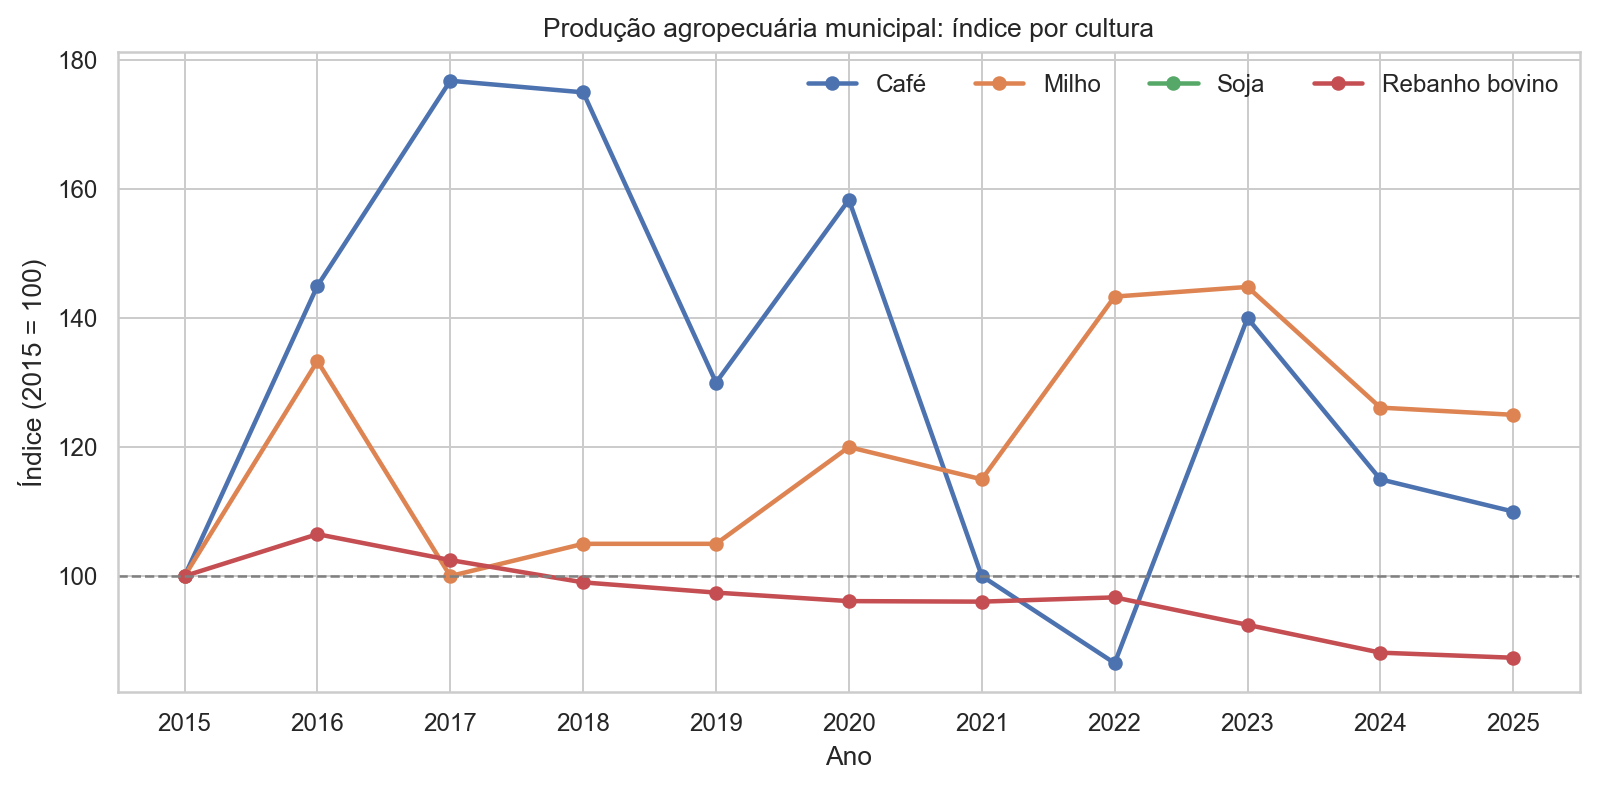
\includegraphics[width=.9\textwidth]{figuras/07_indice_culturas.png}
\caption{Índice de produ\c{c}\~ao agropecu\'aria municipal (2015 = 100).}
\label{fig:indice}
\end{center}
\end{figure}

\section{Discuss\~ao}

Os resultados n\~ao confirmam a hip\'otese de que a chuva anual explica o rendimento do caf\'e em Varginha. Isso n\~ao contradiz a literatura: Victorino \cite{victorino2015} e Aparecido et al.\ \cite{aparecido2016} obtiveram modelos \'uteis ao empregar vari\'aveis de d\'eficit h\'idrico e m\'ultiplas janelas mensais, com s\'eries mais longas e dados de esta\c{c}\~oes ou cooperativas locais. Gomes et al.\ \cite{gomes2026} encontraram correla\c{c}\~oes de sinais opostos entre unidades pr\'oximas no Sul de Minas, o que refor\c{c}a a conclus\~ao de que o efeito do clima \'e local e n\~ao capturado integralmente por uma \'unica esta\c{c}\~ao.

A dire\c{c}\~ao negativa da temperatura na flora\c{c}\~ao e a dire\c{c}\~ao positiva da chuva de janeiro s\~ao coerentes com a fenologia descrita por Meireles e Japiass\'u \cite{meireles2009}. Contudo, com onze observa\c{c}\~oes anuais, o poder estat\'istico \'e baixo: na correla\c{c}\~ao de Spearman, seria necess\'ario um coeficiente pr\'oximo de 0,6 para atingir signific\^ancia a 5\%. Assim, a aus\^encia de signific\^ancia n\~ao prova a aus\^encia de efeito; apenas indica que os dados n\~ao permitem detect\'a-lo.

O epis\'odio dos meses com precipita\c{c}\~ao zero ilustra uma li\c{c}\~ao metodol\'ogica mais ampla. Sem a imputa\c{c}\~ao, o rebanho bovino parecia responder \`a chuva do ano anterior com $R^2=0{,}54$ e $p=0{,}015$; ap\'os a corre\c{c}\~ao, a associa\c{c}\~ao desapareceu. Em s\'eries curtas, uma \'unica falha de sensor pode dominar os resultados. Recomenda-se, portanto, que pipelines p\'ublicos registrem explicitamente quais observa\c{c}\~oes foram imputadas e forne\c{c}am uma an\'alise de sensibilidade.

Entre as limita\c{c}\~oes, destacam-se: uma \'unica esta\c{c}\~ao, que n\~ao representa a heterogeneidade espacial do munic\'ipio; 19 meses imputados, oito em 2023; o descompasso entre o ano civil do SIDRA e o ciclo agr\'icola do caf\'e; vari\'aveis de confus\~ao n\~ao observadas, como pre\c{c}o, \'area colhida, tecnologia, pragas e bienalidade; e o car\'ater preliminar dos dados de 2025. A an\'alise de janelas mensais envolve doze testes e sofre com multiplicidade de compara\c{c}\~oes.

\section{Conclus\~ao}

Este trabalho apresentou uma integra\c{c}\~ao reproduz\'ivel de dados clim\'aticos e agropecu\'arios p\'ublicos para Varginha/MG no per\'iodo de 2015 a 2025. N\~ao foi poss\'ivel detectar efeitos significativos do clima sobre o rendimento anual do caf\'e nem sobre o rebanho bovino. A contribui\c{c}\~ao metodol\'ogica est\'a no c\'odigo aberto, que documenta a leitura dos dois layouts do INMET, a detec\c{c}\~ao de falhas de sensor, a jun\c{c}\~ao via API SIDRA, as janelas fenol\'ogicas e os testes estat\'isticos.

Como trabalhos futuros, recomenda-se ampliar a s\'erie temporal, incluir esta\c{c}\~oes vizinhas e balan\c{c}o h\'idrico, modelar explicitamente a bienalidade da safra e avaliar a sensibilidade dos resultados a diferentes regras de imputa\c{c}\~ao.

\section*{Agradecimentos}

Os autores agradecem ao INMET e ao IBGE pela disponibiliza\c{c}\~ao dos dados p\'ublicos e \`a comunidade de software livre pelas ferramentas utilizadas.

\section*{Declaration of AI-Assisted Use in Writing}
Durante a reda\c{c}\~ao deste artigo, ferramentas de intelig\^encia artificial generativa foram utilizadas apenas para apoio \`a revis\~ao lingu\'\i stica, \`a formata\c{c}\~ao e \`a organiza\c{c}\~ao do texto. Os autores revisaram criticamente todo o conte\'udo gerado ou alterado, conferiram as cita\c{c}\~oes e os resultados e assumem responsabilidade integral pelo texto final. Nenhum dado, figura ou resultado cient\'\i fico foi gerado ou modificado por intelig\^encia artificial.

\bibliography{artigo_bib}

\end{document}
